% !TeX TS-program = xelatex
% !TEX root = main.tex

% How to:
%


% Load class with all definitions. Do not remove this line.
% Options will be passed to Memoir
\documentclass[final]{multiversum}
%

%%%
% Set those variables

% Authors of the document.
% e.g. Max Mustermann, Erika Musterfrau
\multiauthor{Paul, Frieder, Jan, Hanna, Don, Ira}

% Date of release.
% e.g. 31.12.2074
% \multidate{310.03.2020} %306 Tage vom letzten Jahr + Tage in 2021
\multidate{März 2020} % das übliche Format?
% auch wenn ich genrell für full-date (nach RFC 3339) wäre … wobei ein ausgeschriebener Monat schon hübsch aussieht {r}

% Number of release, no leading zeros.
% e.g. 15
\multiausgabe{20}

% Losung
% e.g. Die Kuh lief um den Teig.
\multilosung{Immerhin bist du kein Pferd, sonst wärst du jetzt tot.}


% Logo
% Use a different logo. Defaults to Ueberschrift.svg
%\multilogo{Ueberschrift_xmas}

%
%%%

%%%%%%%%%%%%%%%%%%%%%%%%%%%%%%%%% DOCUMENT %%%%%%%%%%%%%%%%%%%%%%%%%%%%%%%%%
\begin{document}

\makemultititle
%

% PUT BODY HERE
\section{Was bisher geschah...}

\subsection{Jahresrückblick 2020}
Was im letzten Jahr so alles passiert ist, kann man gut zusammenfassen: Alles und nichts.
Eine Klopapierapokalypse ist auf uns niedergefahren und mit ihr eine tödliche Todeskrankheit des Todes +2.
Oder war das andersherum?
Da man sich seit dem März 2020 in seiner Wohnung verbarrikadiert hat, die Barrikaden natürlich aus feinstem Klopapier gefertigt, ist das mit der Außenwelt so ein Ding.
Wärend man sich normalen Tätigkeiten widmet, wie alleine Mehlparties zu schmeißen und reizüberflutet mit den Kollegen zu telefonieren, hat das Rollenspiel eine Kriese.

Soll man sich mit seiner Rollenspielgruppe treffen, während man von seinen Eltern weicht, als wären sie giftig?
Die Melancholie dieser Frage hat uns dieses Jahr sehr bewegt und zu unterschiedlichen Ergebnissen geführt.
Viele Runden wurden in die digitale Welt verschoben und das hat ihnen mehr oder weniger gut getan.
Während Characterplayer sich um das Spielgefühl betrogen fühlen, sind Dungeon Crawl-Fans von den technischen Möglichkeiten durchaus angetan.
Fog of War im Reallife? Awesome! (Ja, Reallife, so nennt sich die digitale Welt jetzt.)

Während das Spiel sich zwangsweise mit unseren neuen Gewohnheiten wandelt, so ist es doch nur anders.
Besser, schlechter? Das muss jeder für sich entscheiden.
Nur eines ist Gewiss:
Was macht das verbrannte Essen meiner Mitbewohner weniger giftig als die Kekse von meiner Oma?
Ach ja, da war so eine Seuche.
\verfasser{Hanna}

\subsection{In der Redaktion}
Montagmorgen, 8 Uhr.
Ich komme in die Redaktion des Multiversums, in der Hand einen Coffee to go.
Huch. Niemand hier? *gähn*
Ich schaue auf die Uhr, Zeit und Datum stimmen.
Alles ist still und wirkt verlassen.

Heute sollte ich zum Jahresbeginn auch mein neues Praktikum beginnen.
Es hieß, ein anderer Praktikant solle mich empfangen und einführen, während die Belegschaft auf einem alljährigen Ausflug in die Multiversen ist.
In Rittersälen zu speisen wäre mir jetzt auch lieber, aber man braucht ja was für den Lebenslauf.
Der Andere ist bestimmt zu spät oder hat mich vergessen.
Professionell betrachte ich den nahezu leeren Eingangskorb.
Darin sind ein Angebot für eine Genitalverlängerung (zum Papierkorb) und eine Rechnung (in den Korb der Verwaltung).
Der Kaffee wird aufgesetzt.
Jetzt müsste mich jemand weiter anleiten.
Unschlüssig setze ich mich an einen zufälligen Schreibtisch und lasse meinen Blick darüber schweifen.
Zwei Monitore, eine Tastatur und Maus, ein Foto eines Loveinterests, ein verdorrter Kaktus.
Über allem liegt eine fingerdicke Staubschicht.
Puh, wo sind die denn alle?
Ich öffne unbeobachtet die Schreibtischschubladen, finde aber keine Hinweise.
Auf einem Notizzettel steht:
\textit{\enquote{Erinnert mich daran, was über Sirenen zu schreiben. Sirenen singen nur beruflich, nicht in ihrer Freizeit.}}
Ich schüttle den Kopf, das ist nicht hilfreich.

Ich stehe wieder auf und streife durch das verlassene Gebäude.
Hinter dem großen Büro mit mehreren Schreibtischen liegt eine Teeküche, jetzt mit fertigem Kaffee.
Daneben gibt es eine Toilette und eine sehr kleine Tür mit einer Maus darauf.
Etwas weiter im Gang, hinter ein paar einzelnen Büros, scheint Licht zu brennen.
Ich halte mich etwas gerader, da ist also doch jemand.
Als ich das Licht erreiche, strahlt es aus einem gläsernen Sitzungsraum.
Über einem langen Holztisch ist ein kleiner Ring auf einem Dreifuß aufgebarrt, aus dem das Licht strömt und das Zimmer erhellt.
Neugierig öffne ich die Schiebetür zum Raum, wobei mir die Tintenflecken auffallen, die das Glas von innen verunstalten.
Um den Tisch herum liegen knitterige Papiere verteilt und mein Haar wird von einem Windstoß zerzaust, der durch den Raum fegt.
Als ich mich dem Licht nähern will, öffnet sich plötzlich neben mir ein violettes Portal, durch das ein Jüngling seinen Kopf steckt.

\enquote{Mist, ist hier richtig?}

Er schaut sich um, erbleicht, als er mich sieht, und streckt die Hand nach mir aus.

\enquote{Bist du die neue Praktikantin? Ich soll dich eigentlich einführen, aber ich hab Scheiße gebaut. 
Komm, wir müssen das fixen, bevor es jemand merkt!}

Zögerlich strecke ich ihm die Hand entgegen, da ergreift er sie schon und zieht mich durch das Weltenportal.
\Verfasser{Die Praktikantin}
\vfill
% \vfill % <- optional, to prevent overly large spacing between paragraphs {r}

\subsection{Anmeldung Weltenbrücken}
Am 30. Januar habt ihr erneut die Chance, das Multiversum vor der vollständigen Zerstörung zu bewahren. 
Da das Weltenbrücken-Rollenspiel dieses Jahr nicht auf der Freusburg stattfinden konnte, öffnen wir die Anmeldung für alle Interessierten, egal ob ihr an der Freizeit teilgenommen hättet oder nicht. 
In den letzten zwei Jahren mussten Quallen zu einem Riss gebracht und verschiedene Aufgaben gelöst werden, was passiert wohl dieses Jahr?
Wenn ihr Lust habt mitzumachen, meldet euch verbindlich bis zum 8. Januar, 18:00 Uhr mit einer Mail an \href{mailto:vorstand@rpg-librarium.de}{vorstand@rpg-librarium.de} (damit wir wissen, wie viele Leute mitspielen wollen).
Das Event selbst findet am 30. Januar von 14-18 Uhr digital über Jitsi Meet statt.
% aahrg, es ist Jitsi Meet, nicht Jitsi ... Jitsi ist der multi-Protokoll-Client! (https://github.com/jitsi/jitsi) {r}
\verfasser{Jan}

\subsection{Freizeit in der Freizeit}
Wie so vieles in diesen Zeiten muss zu unserer großen Enttäuschung auch die Librariumspräsenzfreizeit 2021 wegfallen.
Während wir in unseren behaglichen Nestern hocken und die Knochenkälte der Burg vermissen, können wir uns etwas Abhilfe schaffen.
Am ersten Januarwochenende gab es eine kleine digitale Freizeit.
Unser großartiger Vorstand hat uns dafür einen Discordserver eingerichtet, der einige Spieltisch- und Workshopchannels beinhaltet.
Es sind dabei ein paar gesellige Spielrunden zustande gekommen und auch der Tavernenchannel war zu den meisten Tageszeiten rege besucht.
Es gab Diskussionen über Regeln, die Relation zu den eigenen Charakteren und Buchcover mit nackten Oberkörpern.
Der ein oder andere soll auch einen Charakter gezeichnet haben.
Trotz aller Widernisse war die Onlinefreizeit ein guter Jahresbeginn und der Server besteht noch bis zum Ende der Woche.
Fürs nächste Jahr hoffen wir aber wieder auf frierende Burgmauern.
\verfasser{Hanna}
% ^ hier evtl Verfasser statt verfasser? Das ist ein wenig eng ... {r}
% TODO: consider adding an em quad/space before the name in \verfasser (cls file) {r}
% \vspace{-.5 \baselineskip}

\begin{figure}[h]
  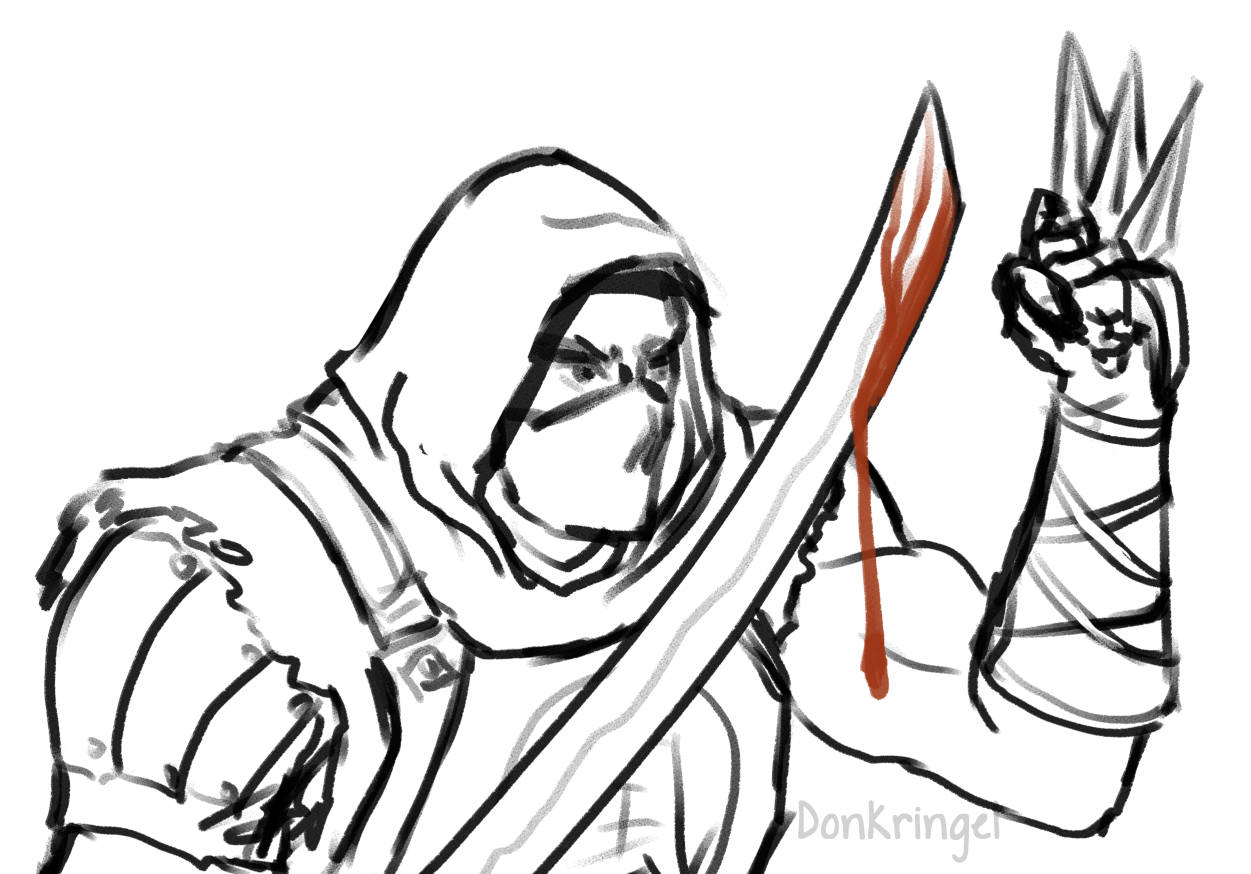
\includegraphics[width=0.45\textwidth]{src/img/ninja_assassin_rache_for_multiversum.jpg}\\
  Viele Tote \emph{fast} ohne Zeugen.
  Rache, ein Charakter aus der Savage Worlds Ninja Assassin Runde, gespielt auf der Digitalfreizeit.
\end{figure}
\vspace{-1 \baselineskip}

\begin{termine}
% Put dates here:
\item Monatliches Treffen: 16.01.2021, 19 Uhr
\item Weltenbrücken: 30.01.2021, 14-18 Uhr
\end{termine}

\section{An einem anderen Ort}

\subsection{Zwei Tote in Hetta}
In den vergangenen Tagen wurden zwei tote Touristen in Hetta, Lappland gefunden. 
Die finnische Polizei hat der Oulu Sanomat versichert, dass sie den Todesfällen mit Nachdruck nachgehen. 
Die erste Leiche wurde in der Nähe der örtlichen Skipisten gefunden. 
Die zweite Leiche wurde nahe der touristischen Attraktion \textit{Hetta Huskies} gefunden.
Die Polizei vermutet, dass die Opfer einem wilden Wolfsrudel zum Opfer fielen. 
Diese sind in Lappland nur noch selten anzutreffen. 
Touristen wird von der Polizei empfohlen, sich vom Wald fern zu halten, bis die Lage geklärt wurde. 
Der Bürgermeister des Ortes erklärte, dass er sich für die Biodiversität der Region einsetze, aber die Sicherheit der Menschen ebenfalls gewährleistet sein muss. 
Der Pastor der Gemeinde hat angekündigt, kommenden Sonntag eine Trauerpredigt zu halten.
\zeitung{Oulu Sanomat, 20. tammikuu 2020}
\verfasser[Werewolf: The Forsaken]{Ira}

\subsection{Herbert @herbwest}
That moment. Als Tourist durch Innsmouth kommen und merken, dass die eigene Familie da her kommt. \#deep
\zeitung{5:12am $\cdot$ 23th May 1929}
\verfasser[Cthulhu]{Hanna}

\subsection{Firenzes Panoptikum fabuloser Tinkturen}
Hühneraugen, Warzenweyden, Schmerzensreygen\\
Firenze Fabuloso heilt so ziemlich jedes Leyden!\\
Liebesleyd und kalter Schart oder sogar Alkehyst,\\
Firenze Faboloso weiß wie man's bemisst!\\[\baselineskip]
Extravagante Tinkturen zu annehmbaren Preisen.\\
Bald in Ihrer Stadt, nur für kurze Zeit! 
\verfasser[DSA5]{Frieder}

\section{Schleuderpresse}
\textit{Hier könnte deine Gruppensuche stehen, schreib uns an \href{mailto:multiversum@rpg-librarium.de}{multiversum@rpg-librarium.de}! 
Steht kein Kontakt bei einer Anzeige? Dann schreib der Redaktion mit dem Zeichen im Betreff}

\subsection{Finde deinen Weg mit einer Pathfinder Runde}
Gruppe von 4 suchen Spieler*innen mit Interesse für Rollenspiel, für gemütliche Pathfinder Abende zusammen.
Wir sind bilingual, offen für eine neue (schwebende) Welt.
\verfasser{5.4.-311}
\zeichen{Revolution}
\Verfasser[Pathfinder]{Paul} % haben wir das üblicherweise mit angegeben? {r}

\impressum

\end{document}
%%%%%%%%%%%%%%%%%%%%%%%%%%%%%%%%% END DOCUMENT %%%%%%%%%%%%%%%%%%%%%%%%%%%%%%%%%
